\documentclass[sigconf]{acmart}

\usepackage{booktabs} % For formal tables

\newif\iffinal

% Un-comment this line to see proposal without comments
%\finaltrue

\iffinal
  \newcommand\ian[1]{}
  \newcommand\kyle[1]{}
  \newcommand\eli[1]{}
  \newcommand\bb[1]{}

\else
  \newcommand\ian[1]{{\color{blue}[Ian: #1]}}
  \newcommand\kyle[1]{{\color{red}[Kyle: #1]}}
  \newcommand\eli[1]{{\color{green}[Eli: #1]}}
  \newcommand\bb[1]{{\color{violet}[Blaiszik: #1]}}
\fi

% Copyright
%\setcopyright{none}
%\setcopyright{acmcopyright}
%\setcopyright{acmlicensed}
\setcopyright{rightsretained}
%\setcopyright{usgov}
%\setcopyright{usgovmixed}
%\setcopyright{cagov}
%\setcopyright{cagovmixed}

% DOI
\acmDOI{10.475/123_4}

% ISBN
\acmISBN{123-4567-24-567/08/06}

%Conference
\acmConference[PDSW-DISCS 2017]{2nd Joint International Workshop on Parallel Data Storage \& Data Intensive Scalable Computing Systems}{November 2017}{Denver, Colorado USA} 
\acmYear{2017}
\copyrightyear{2017}

\acmPrice{15.00}


\begin{document}
\title{Petrel: A Programmatically Accessible Research Data Service}

\author{Benjamin Allen, William Allcock, Rachana Ananthakrishnan,\\Ben Blaiszik, Kyle Chard, Ian Foster, Lukasz Lacinski, and Michael Papka}
\affiliation{%
  \institution{Argonne National Laboratory}
  \streetaddress{9700 S Cass Ave, Lemont, IL 60439, USA}
%  \city{Lemont} 
%  \state{IL} 
%  \postcode{60439}
}
\renewcommand{\shortauthors}{B. Allen et al.}


\begin{abstract}

Data-intensive science requires new data services beyond those provided by conventional
high-performance computing (HPC) systems.
We established the Petrel data server at Argonne National Laboratory in 2015 to experiment with the utility and operation of such services.
This high-capacity, high-speed data store was configured to enable both interactive Web access
and programmatic access via REST APIs and associated 


Petrel is a data management service operated by the Argonne Leadership Computing Facility (ALCF)
that allows researchers to store large datasets and easily share those data with collaborators. 
%Researchers from the Argonne Leadership Computing Facility (ALCF) and Globus are developing the system collaboratively. 
Petrel leverages ALCF
storage and infrastructure and Globus transfer and sharing services to provide a mechanism for researchers to transfer data into the system, manage data on the filesystem, and share and transfer data to other locations. Authentication and identity to access the system is provided through Globus and users can access Petrel using their campus or institution federated login.
We report here on the design, implementation, applications, and use of this service.
\textbf{The paper is to be submitted to \url{http://www.pdsw.org/index.shtml}. Five pages plus references. Due September 7, 11:59 PM, AOE.}
\end{abstract}

%
% The code below should be generated by the tool at
% http://dl.acm.org/ccs.cfm
% Please copy and paste the code instead of the example below. 
%
\begin{CCSXML}
<ccs2012>
 <concept>
  <concept_id>10010520.10010553.10010562</concept_id>
  <concept_desc>Computer systems organization~Embedded systems</concept_desc>
  <concept_significance>500</concept_significance>
 </concept>
 <concept>
  <concept_id>10010520.10010575.10010755</concept_id>
  <concept_desc>Computer systems organization~Redundancy</concept_desc>
  <concept_significance>300</concept_significance>
 </concept>
 <concept>
  <concept_id>10010520.10010553.10010554</concept_id>
  <concept_desc>Computer systems organization~Robotics</concept_desc>
  <concept_significance>100</concept_significance>
 </concept>
 <concept>
  <concept_id>10003033.10003083.10003095</concept_id>
  <concept_desc>Networks~Network reliability</concept_desc>
  <concept_significance>100</concept_significance>
 </concept>
</ccs2012>  
\end{CCSXML}

\ccsdesc[500]{Computer systems organization~Embedded systems}
\ccsdesc[300]{Computer systems organization~Redundancy}
\ccsdesc{Computer systems organization~Robotics}
\ccsdesc[100]{Networks~Network reliability}


\keywords{TBD, TBD, TBD}


\maketitle

We report on our experiences deploying and operating Petrel,
a high-speed data service designed to support science projects 
that must acquire, organize, and distribute large quantities of data.
By integrating a high-speed, highly connected, and programmatically
controllable data store within the fabric of a data-rich science
environment, we sought to   


Petrel's primary innovation is its use of Globus REST APIs to enable
secure, reliable programmatic access to, and management of, 

Building on a base of a high-speed 1.7~PB parallel file system, Petrel
innovates in its use of Globus REST APIs to enable programmatic control

Data-intensive science increasingly requires discipline-based data management tools,
for example to distribute content from a curated repository, 
share files from a computational simulation or scientific instrument with remote collaborators,
enable analyses of hosted data by remote collaborators, 
or accept uploads for analysis or publication.
Traditional high-performance computing facilities \bb{Repeated below in Introduction}

Petrel represents one sort of expansion of what is traditionally thought of as the role of high-performance computing facilities~\cite{UrPa16}. 
This is in addition to providing a large supercomputers for running traditional simulations, 
facilities need to evolve to become a highly usable service facility, 
deeply integrated into science projects and serving as a hub for science communities. 
Petrel introduces a new service that integrates with user environments and workflow to improve the usability and utilization of HPC centers. 
It provides a configurable solution to the sharing of data with colleagues and the community, 
while at the  same time keeping the large datasets close to large computational resources.



\section{Introduction}

Data-intensive science increasingly requires discipline-based data management tools,
for example to distribute content from a curated repository, 
share files from a computational simulation or scientific instrument with remote collaborators,
enable analyses of hosted data by remote collaborators, 
or accept uploads for analysis or publication.
But would-be developers of such tools need a foundation on which to build:
a foundation that is not necessarily provided by 
conventional research computing facilities,
which are typically designed to support individual research projects 
rather than long-lived and community services.
They need, in particular,  
storage systems that provide substantial capacity and
high-speed storage and network access,
and that can be managed and accessed entirely programmatically
%(e.g., via REST APIs) 
for easy integration into domain-specific workflows.

These considerations led us to establish the Petrel data service in 2015,
initially as an experiment to see whether and how people
might use a programmatically accessible storage service, 
and then---as success stories emerged---as a production
service for the Argonne community.
The current Petrel system provides Globus REST API  
access to 1.7~PB high-speed storage, 
connected to local and wide area networks
at 100~Gbps.
Authorized users can use Globus APIs (and associated Web interfaces) to  
move files to and from storage and to authorize others to do the same. 

We have found the results of this experiment to be highly encouraging.
Dozens of groups have made use of Petrel in one way or another to transfer
data between Petrel and more than 600 remote locations.
Many groups have integrated its use into workflows, often in innovative
ways that we had not considered. 

We report here on the design, application, and usage of the Petrel system
and reflect on lessons learned from its development and use.

Petrel represents one sort of expansion of what is traditionally thought of as the role of high-performance computing facilities~\cite{UrPa16}. 
This is in addition to providing a large supercomputers for running traditional simulations, 
facilities need to evolve to become a highly usable service facility, 
deeply integrated into science projects and serving as a hub for science communities. 
Petrel introduces a new service that integrates with user environments and workflow to improve the usability and utilization of HPC centers. 
It provides a configurable solution to the sharing of data with colleagues and the community, 
while at the  same time keeping the large datasets close to large computational resources.


%From a slide that I had on Petrel for ALCF review where we called it a data service
%
%�A uniform data fabric across the lab
%� with seamless access to large data�
%� for use in computation, collaboration and distribution �
%� that is project focused and self 
%managed �
%� and is described and discoverable�


%modern research data portal   
%
%Providing such data acceleration services is a natural way for research computing centers to deliver enhanced value to their stakeholders. But implementing and operating such services can be expensive and cumbersome. 
%
%researchers often need to stage, store, share, and distribute large quantities of data.
%In response, we designed and deployed Petrel, 
%a data service designed to support scientific  
%
%programmatic access for automation 
%
%Conventional research computing facilities are rarely well suited for such purposes,
%being designed to support computational projects rather than data distribution.
%for example, a person may need an allocation and account before
%they can access a data system.
%
%Argonne National Laboratory is home to thousands of intramural scientists and also
%operates a variety of scientific user facilities,
%including both experimental apparatus such as the Advanced Photon Source,
%with its more than 60 beamlines, and supercomputers, such as those operated
%by the Argonne Leadership Computing Facility.
%These facilities are used by many thousands of scientists annually, who increasingly
%face the need 
%These facilities and other activities at the lab increasingly involve large 
%quantities of data, 
%which proved to be surprisingly difficult to manipulate due to the lack of suitable storate facilities 
%




%\begin{verbatim}
%32 Nodes with 1.7 PB usable storage
%GPFS and Globus
%100TB allocation per project
%Transfer and sharing data with collaborators
%Federated login
%Self-managed by PIs
%\end{verbatim}

MRDP~\cite{BMRDP}.

DEBD~\cite{foster2015networking}.


%Transfers to/from Petrel 80027
%Transfers from Petrel 59018
%Transfers to Petrel 21304
%Transfers within Petrel 295
%Unique src EPs 281
%Unique dst EPs 522
%Unique EPs 649
%Total data from Petrel 2.07274415613e+15
%Total files from Petrel 72779854.0
%Total data to Petrel 4.13027153675e+15
%Total files to Petrel 255731042.0
%Total data to/from Petrel 6.1187793935e+15
%Total files to/from Petrel 326728415.0

A total of 80,027 transfers (59,018 outbound, 21,304 inbound),
comprising 6.12~PB (2.07~PB outbound, 4.13~PB inbound) and 327M files (73M outbound, 256M inbound).
(Numbers do not add up perfectly due to a few hundred transfers from Petrel to Petrel.)


\section{The Petrel System}

The Petrel system comprises a parallel file system running the
IBM General Parallel File System (GPFS)~\cite{schmuck2002gpfs},
plus eight associated data transfer nodes (DTNs)~\cite{dart2014science} for remote access. 
Globus services are used to manage access, data transfers, and data sharing.

\begin{figure}
\centering
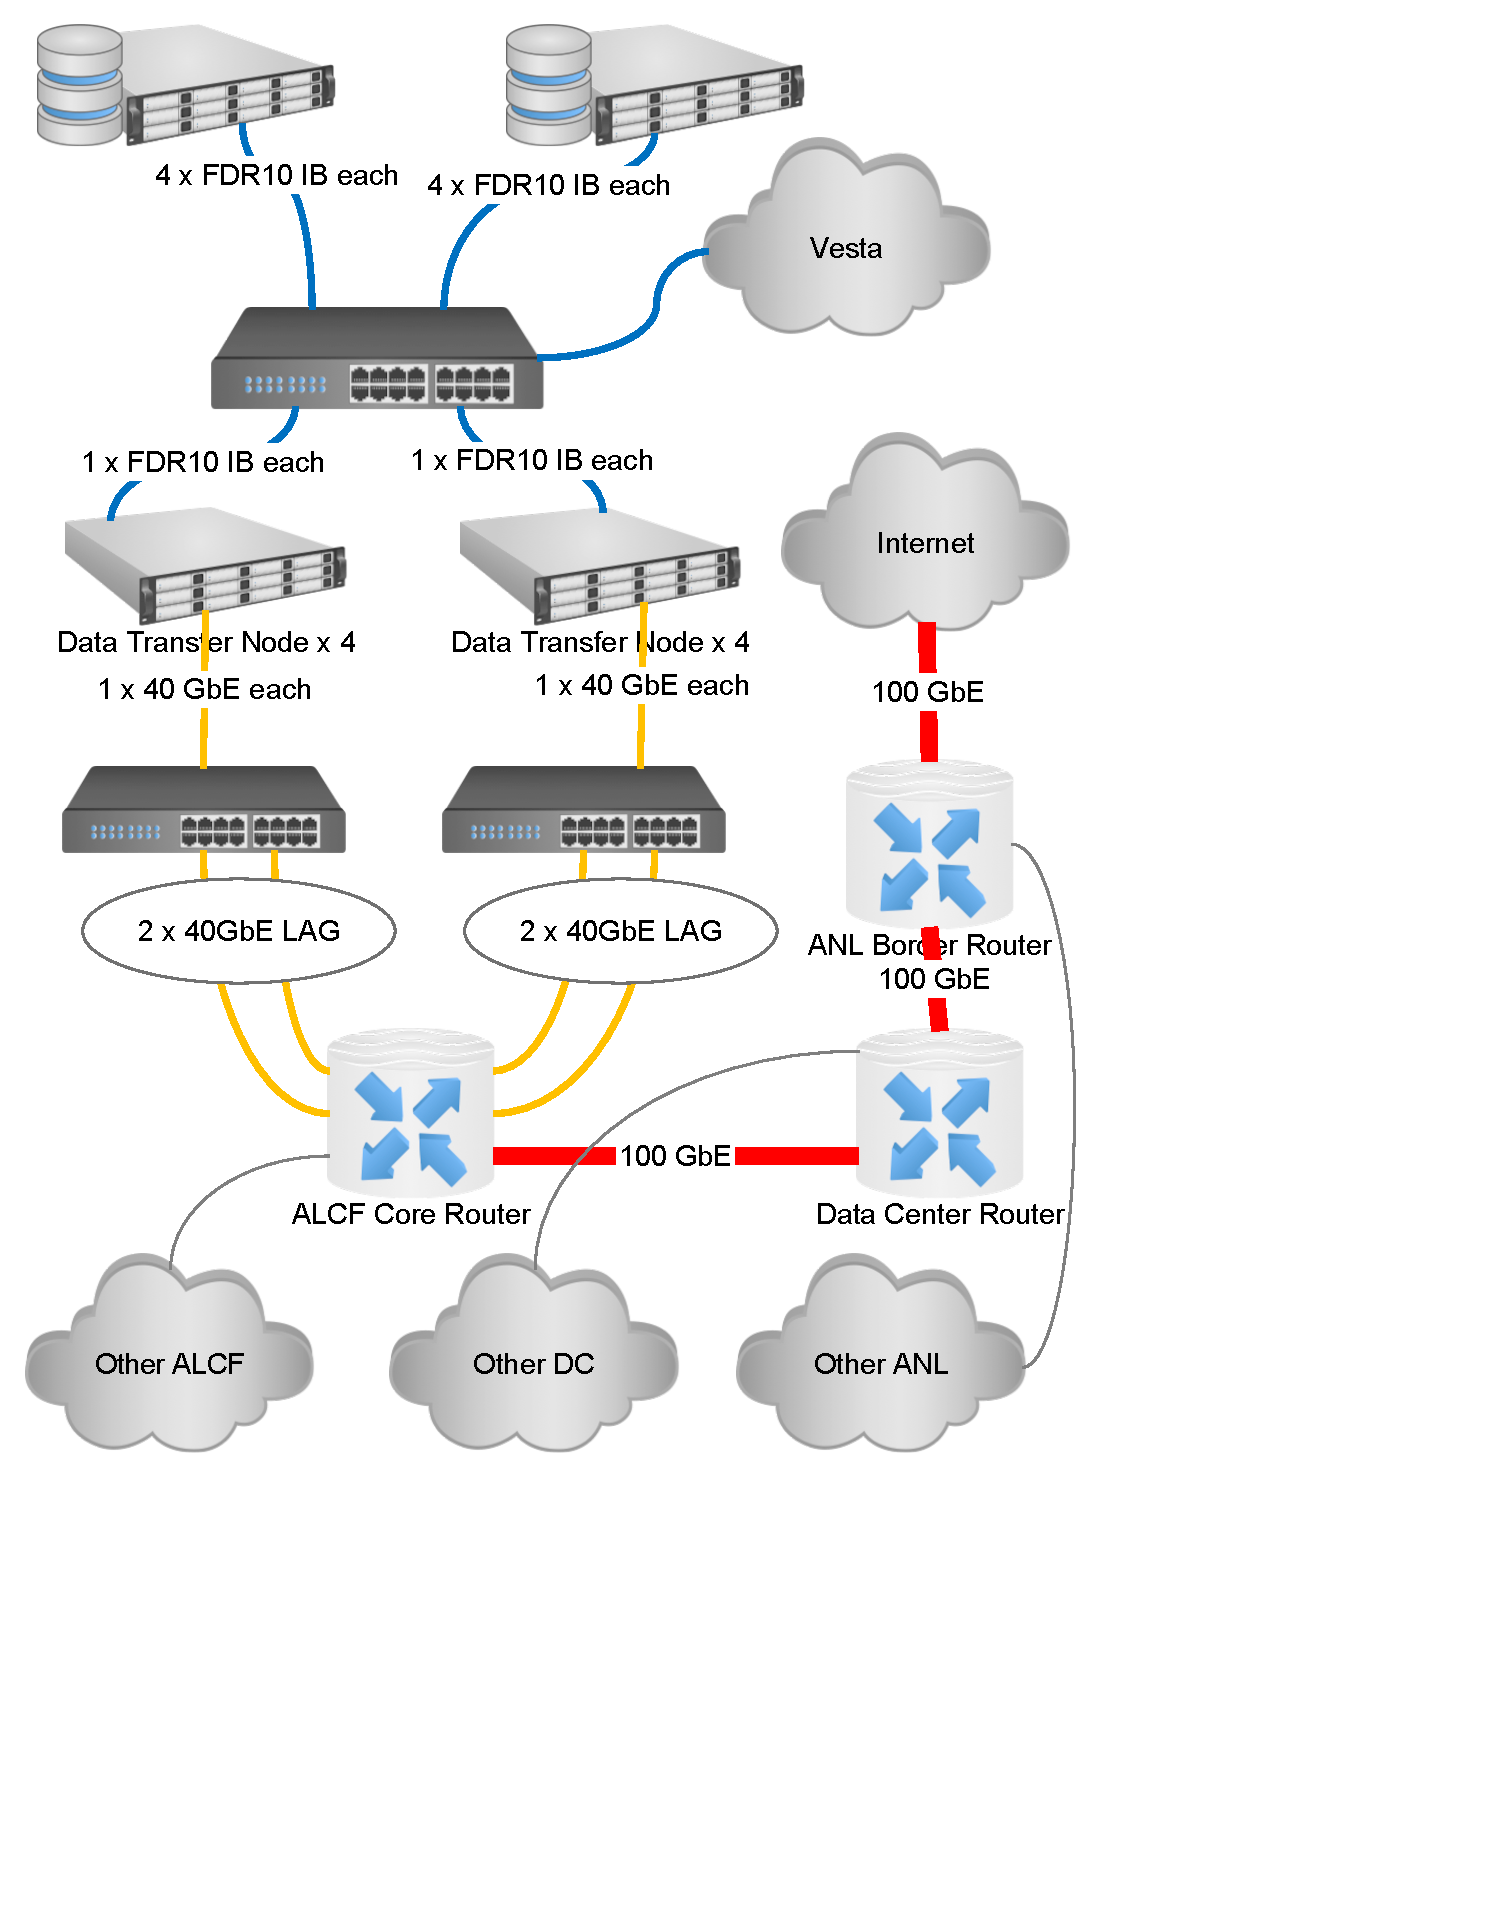
\includegraphics[trim=0.1in 3in 2.7in 0,clip,width=\columnwidth]{Figures/PetrelSystemDiagramNarrow.pdf}

\vspace{-1ex}

\caption{Petrel architecture, as described in the text. The NSD servers are at the top,
with the DTNs are below them. The remainder of the figure shows how Petrel is connected to
ALCF, other data center, and remote networks. \label{fig:arch}}
\end{figure}


\subsection{Hardware: Parallel Store and DTNs}

Petrel hardware comprises a single IBM Elastic Storage Server (ESS) GL6 plus eight DTNs for external access.

An ESS GL6 is configured with two IBM S822L Power8 based servers as IBM GPFS Network Shared Disk (NSD) servers, and one IBM S812L as a management and provisioning server. 
Each NSD server is connected with 4$\times$FDR10 connections to the same fabric as the DTNs. 
Petrel includes six disk trays with a total of 348 6TB SAS HDDs. 
Configured with 8+2 parity and 3 drives worth of hot spare space, Petrel provided a usable capacity of 1.7P, and was benchmarked via IOR at Max Write: 16,563.06 MiB/sec (17,367.62 MB/sec), Max Read:  23,110.68 MiB/sec (24,233.31 MB/sec).

Each of the eight Petrel DTNs has a single Mellanox ConnectX-4 40GbE NIC, a single Mellanox Connect-IB HBA (running at QDR), 64GB RAM ($\sim$42GB dedicated to GPFS), and a single socket Intel E5-1660 v3 8c @ 3.00GHz CPU. 
Both Mellanox cards sit on PCIe 3.0 x16 buses.

The eight Petrel DTNs are connected to two core Mellanox SX1710 36-port 40GbE switches
maintained within Argonne's Joint Laboratory for Systems Evaluation (JLSE).
%JLSE has two core Mellanox SX1710 36-port 40GbE switches. 
The Petrel DTNs are split across the two switches, each connected with 1$\times$40GbE. 
%The split is along even and odd numbered DTNs. 
Each of the two 40GbE core switches has a 2$\times$40GbE link aggregation group to the ALCF core router, which in turn has a 100GbE connection to the core router for the data center within
which ALCF is located,
%SDN240. 
%At this point we are sharing available bandwidth with ALCF. 
%SDN240 in turns 
which in turn connects at 100GbE to one of the ANL border routers.
Thus, as Petrel traffic reaches beyond JSLE to ALCF, the data center, and the border,
it shares bandwidth with an increasing range of other activities.
%At this point we share available bandwidth with all of the 240 datacenter, 
%and at the border we share with the rest of the lab to ESNet.

\subsection{Software: GPFS and Globus}

Petrel uses GPFS as its file system. 
Remote access is provided via Globus services~\cite{Globus2016}.
Globus provides data and identity management capabilities designed for the research community. 
These capabilities are delivered via a cloud-hosted software- and platform-as-a-service model, 
enabling users to access them through their web browser and
developers to invoke them via powerful APIs. 
We describe here Globus capabilities for managing and transferring data and for authenticating users and authorizing access.

Globus allows data to be remotely managed across its pool of more than 10,000 accessible storage systems (called ``endpoints''). 
A storage system is made accessible to Globus, and thus capable of high performance and reliable data transfer, by installing Globus Connect software. 
Globus Connect is offered in two versions: 
Globus Connect Personal for single-user deployments (e.g., a laptop or PC) and Globus Connect Server for multi-user
deployments (e.g., a shared server or DTN). 
Petrel runs Globus Connect Server software.

Globus Transfer capabilities provide high performance and reliable third party data transfer. 
The Globus service manages the entire transfer process, including coordinating authentication at source and destination; establishing a high performance data channel using  the GridFTP protocol, with configuration optimized for transfer; ensuring data integrity by comparing source/destination checksums; and recovering from any errors during the transfer.  Globus, by default, enforces the data access permissions represented
by the underlying system; however, it also allows these access decisions to be managed through the cloud service. In the latter mode, called Globus Sharing, users may associate user- or group-based access control lists (ACLs) with particular file paths. Globus checks and enforces these ACLs when other users attempt to read or write to those paths.

Globus Auth provides identity and access management platform capabilities. It brokers authentication and authorization interactions between end-users, identity providers, resource servers (services), and clients (e.g., web, mobile, desktop, and command line applications, and other services). 
It implements standard web protocols, such as OAuth 2.0 and OpenID Connect, that allow it to be integrated easily with external applications using standard client libraries. 
These protocols enable third-party applications to authenticate users (using their preferred identity) directly with the chosen identity provider. Globus Auth then returns access
tokens that the third-party application can use to validate the user's identity and to perform actions on behalf of that user, within an agreed upon scope. Globus Auth implements an identity federation model via which diverse identities can be linked, and such that presentation of one identity may support authorization for the set of identities. Integration with Globus Groups supports group-based authorization using user-managed groups.



\section{Example User Workflows}

Beamline scientists from Argonne's Advanced Photon Source (APS) use Petrel as a resource for their data management.

A scientist requests a project allocation on Petrel. 
Upon approval, they have access to 100TB. 
They also have the right to add other users, 
to whom they can grant rights to manage, read, and/or write the space.

Once data is generated at APS, scientists transfer it to the project space on Petrel. 
They can then set up permissions to enable remote collaborators to access all or a subset of the data. 
Importantly, remote collaborators do not need Argonne accounts to access the data.

Petrel users can easily stage all or some of their data to a compute resource for analysis, and then move results back to Petrel.

\subsection{Tomography}

A microtomography research team at Argonne's Advanced Photon Source (APS) collects 20--80 TB/month of raw data, and expects to scale to about 100--200 TB/month in the near future. 
Microtomography can be carried out at a variety of energies suitable for 3D characterization of materials relevant to materials science, geoscience, energy storage, and biology. 
High-speed imaging allows for ultra-short exposure times, allowing for detailed study of transient material phenomena. 
Researchers in this group get an allocation at the beamline for a duration of a few days, and gather data that needs to be further processed and analyzed. 
Subsets of the raw data need to be moved to a diverse set of analysis and storage facilities for processing and long-term preservation. Users can leverage Petrel to help meet these requirements. 
APS beamline users would also like to use Petrel to track their study metadata and provenance, and share raw and analyzed data with collaborators (some working remotely).

Things that mention Petrel: Tekin paper~\cite{bicer2016optimization}. Skluma~\cite{beckman2017skluma}.

\subsection{Materials Science}

A group of scientists from Argonne's Materials Science Division (MSD) gather experimental data from APS beamlines with raw data volumes ranging from 60--100 TB/month with data volumes expected to double by 2016. These scientists require a flexible environment to implement end-to-end experiment-time data analysis workflows to automate their analyses and leverage distributed computing resources. This functionality allows the researchers to compare their experimental data to simulation results drawn from high-performance computing resources to rapidly provide actionable feedback and data visualization. These scientists can leverage Petrel to help meet these requirements.

Through Petrel and Globus functionality, we provide intuitive interfaces for these researchers to share, bundle, and publish their datasets. After data is gathered, the scientists often want to share subsets of raw data, derived datasets, and analysis results with collaborators, track metadata associated with the data, and track data provenance. Eventually, these scientists may want to make their datasets publicly and persistently available via publication functionality, fully bundled with the associated metadata and associated with a persistent identifier to aide search, discovery, and data citability.

The Materials Data Facility (MDF)~\cite{MDF2016} is an effort to build production data services for the materials science community
to enable simplified publication, discovery, and reuse of materials-related datasets. The MDF data publication service allows researchers to 
publish datasets stored on distributed resources (i.e., any Globus endpoint), mint permanent unique identifiers 
(e.g., DOI or Handle), and implement data publication workflows through a web UI or an API. The MDF data discovery service provides 
a simple API and python tools to help users to query and access full datasets published in MDF as well as a host of data and metadata indexed 
from a variety of external efforts (117 sources indexed to date). 

MDF leverages the flexibility of the Petrel service in a variety of ways including: 
1) sharing collaborative spaces with research teams across the country for use in collaboratively collecting project 
data prior to final publication and sharing with the public;
2) staging all datasets to Petrel for indexing into the discovery service (currently comprises ~60 TB of data); and
3) storing a raw copy of the extracted JSON-formatted metadata for index persistence. In the 
future, MDF is interested in attaching compute resources to Petrel in order to facilitate more simple operation on  
the stored datasets. These operations may include, e.g., indexing, analyzing, visualizing, submitting jobs to other
ALCF resources, or interacting with the data via applications such as Jupyter.

\section{Usage Data}

A total of 80,027 transfers, of which 59,018 were from Petrel, 21,304 to Petrel, and 295 within Petrel.
A total of 649 unique endpoints engaged in communication with Petrel, 281 as sources and 522 as destinations. 

%Here are the stats you asked for:
% 
%Transfers to/from Petrel: 80027
%Transfers from Petrel: 59018
%Transfers to Petrel: 21304
%Transfers within Petrel: 295
% 
%Unique from Eps: 281
%Unique to Eps: 522
%Unique Eps: 649
% 
%Eps mapped to location: 639 (/649)
% 
%Transfers
%No to location: 259
%No from location: 885
% 
%Zero km to Petrel: 16133
%Zero km from petrel: 6375
% 
%Total transfers after removing Eps where we don�t have a location and transfers with 0 km distance
%Total to Petrel: 4912 (/21304)
%Total from Petrel: 51758 (/59018)

Another fun fact of this system, since we put it into production we have only had a single hard drive fail, and that was just a few weeks ago. Since it was installed we have only had one additional drive fail, which was during early burn-in.

Here is a list of all Petrel projects (excepting test or demo projects),
disk space usage, with an organization and department of a PI of each
project:

%37T     2idb (Argonne National Laboratory; Advanced Photon Source/X-ray
%Science Division)
%4.3T    ACME (Argonne National Lanboratory; MCS)
%12T     alpha-nek (University of Chicago; Physics)
%3.6T    CODAR (Argonne National Lanboratory; MCS)
%89T     Discovery Engines for Big Data  (Argonne National Laboratory; MCS)
%674M    Discovery Engines LDRD (Argonne National Laboratory;
%MCS/Computation Institute)
%0       ECP-Candle (University of Chicago; CELS)
%13T     EWN (University of Chicago; Computation Institute)
%42T     Fuel Spray (Argonne National Laboratory; XSD/TRR)
%5.6T    gixs (Argonne National Laboratory; Advanced Photon Source)
%195G    Globus (Argonne National Laboratory; MCS)
%0       Globus bandwidth testing (National Institutes of Health; NIH HPC)
%2.4T    globuslabs (University of Chicago; Computation Institute)
%142T    globusperformancetesting (University of Chicago; Globus)
%39G     globuspublish (University of Chicago; Computation Institute)
%0       IMCA data transfer (AbbVie Inc; AbbVie IR)
%51T     NRCM_DD (Argonne National Laboratory; EVS)
%0       Patric (Argonne National Laboratory; CELS)
%59T     Research Data Analytics (Argonne National Laboratory/University
%of Chicago; CELS-Computation Institute)
%53G     RSPrec  (NRL; Plasma Physics)
%38G     SBC-CAT Data Management (Argonne National Laboratory; Advanced
%Photon Source)
%37G     SDM (Argonne National Laboratory; Advanced Photon Source)
%30G     Small Worlds (Argonne National Laboratory; Argonne Leadership
%Computing)
%1.1T    Structural Biology Data Grid (Harvard Medical School; BCMP)
%481T    tomography (Argonne National Laboratory; Advanced Photon Source)
%84T     xbrainmap (Argonne National Laboratory; Advanced Photon Source)
%26T     xfm (Argonne National Laboratory; Advanced Photon Source)
%154T    XPCS (Argonne National Laboratory; Advanced Photon Source)
%0       X-ray ptychography (Argonne/Northwestern; APS)
%
%25 projects (out of all 29) stored data
%Total file system usage: 1.3 PB



\begin{figure}
\centering
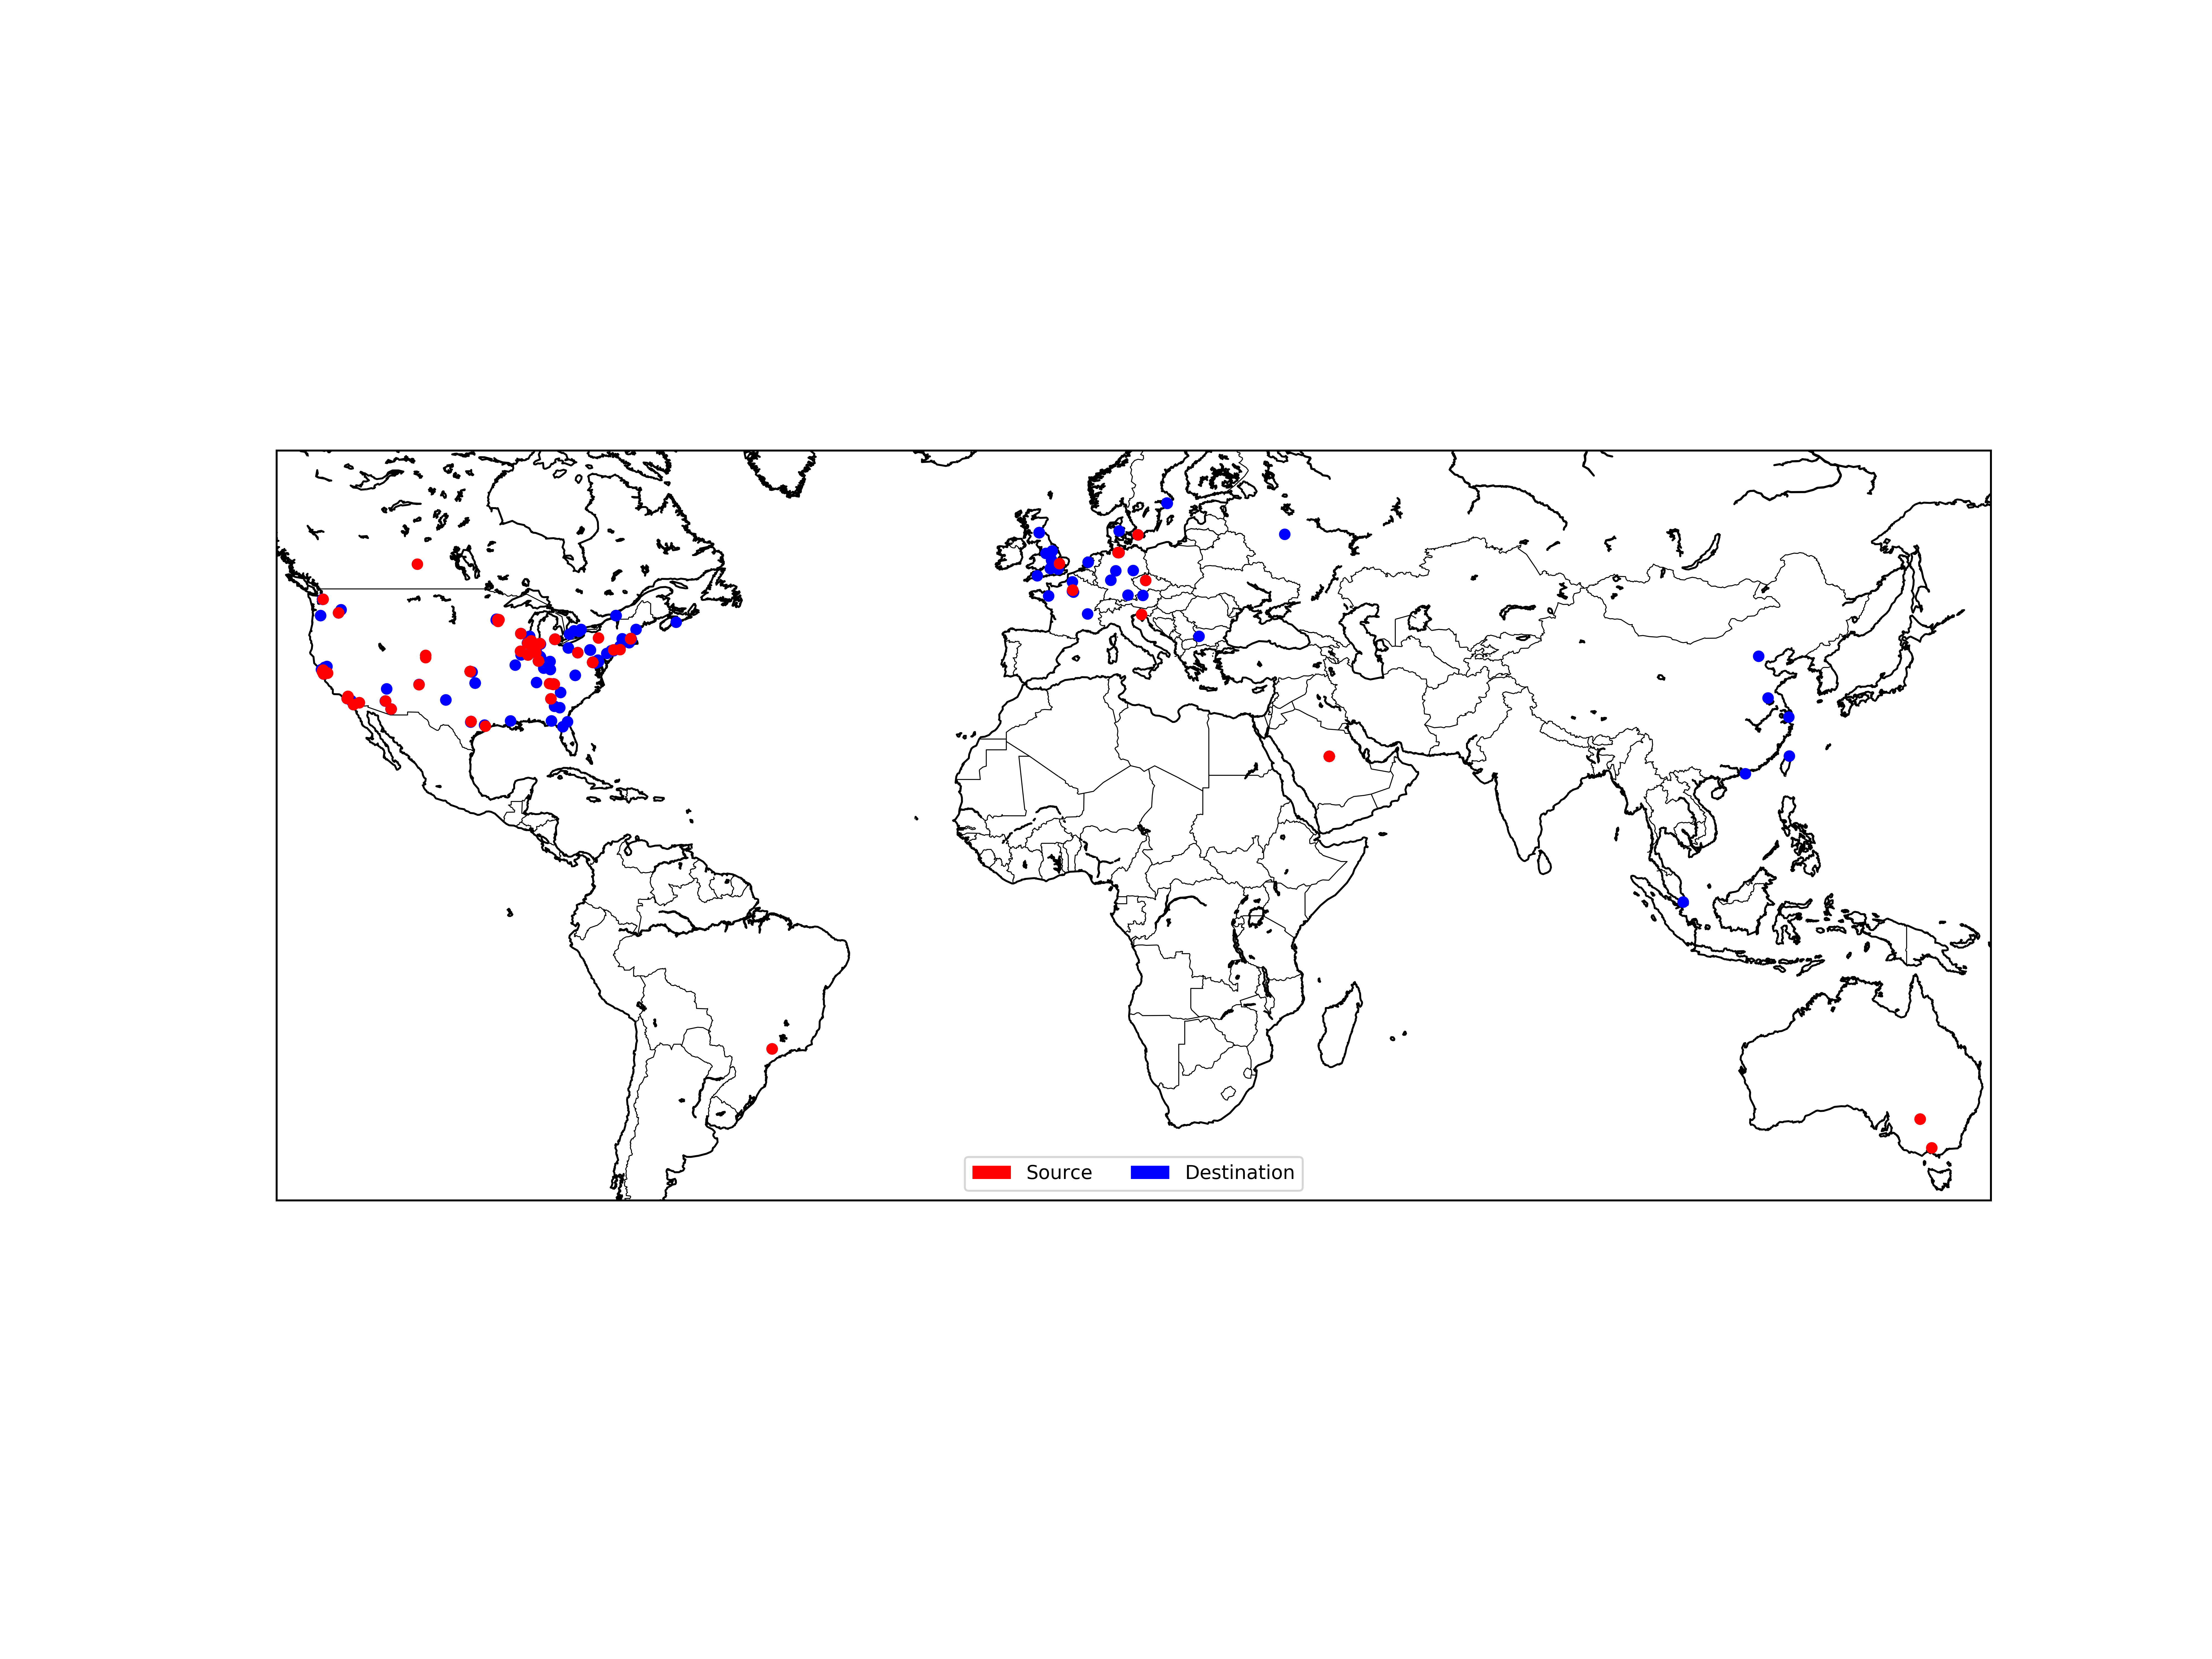
\includegraphics[trim=2in 3.3in 1.4in 3in,clip,width=\columnwidth]{Figures/petrel-src-dst-map2.png}

\vspace{-1ex}

\caption{The 639 (of 649 total) Petrel source and destination endpoints for which geolocation
data are available.\label{fig:usage1}}
\end{figure}


\begin{figure}
\centering
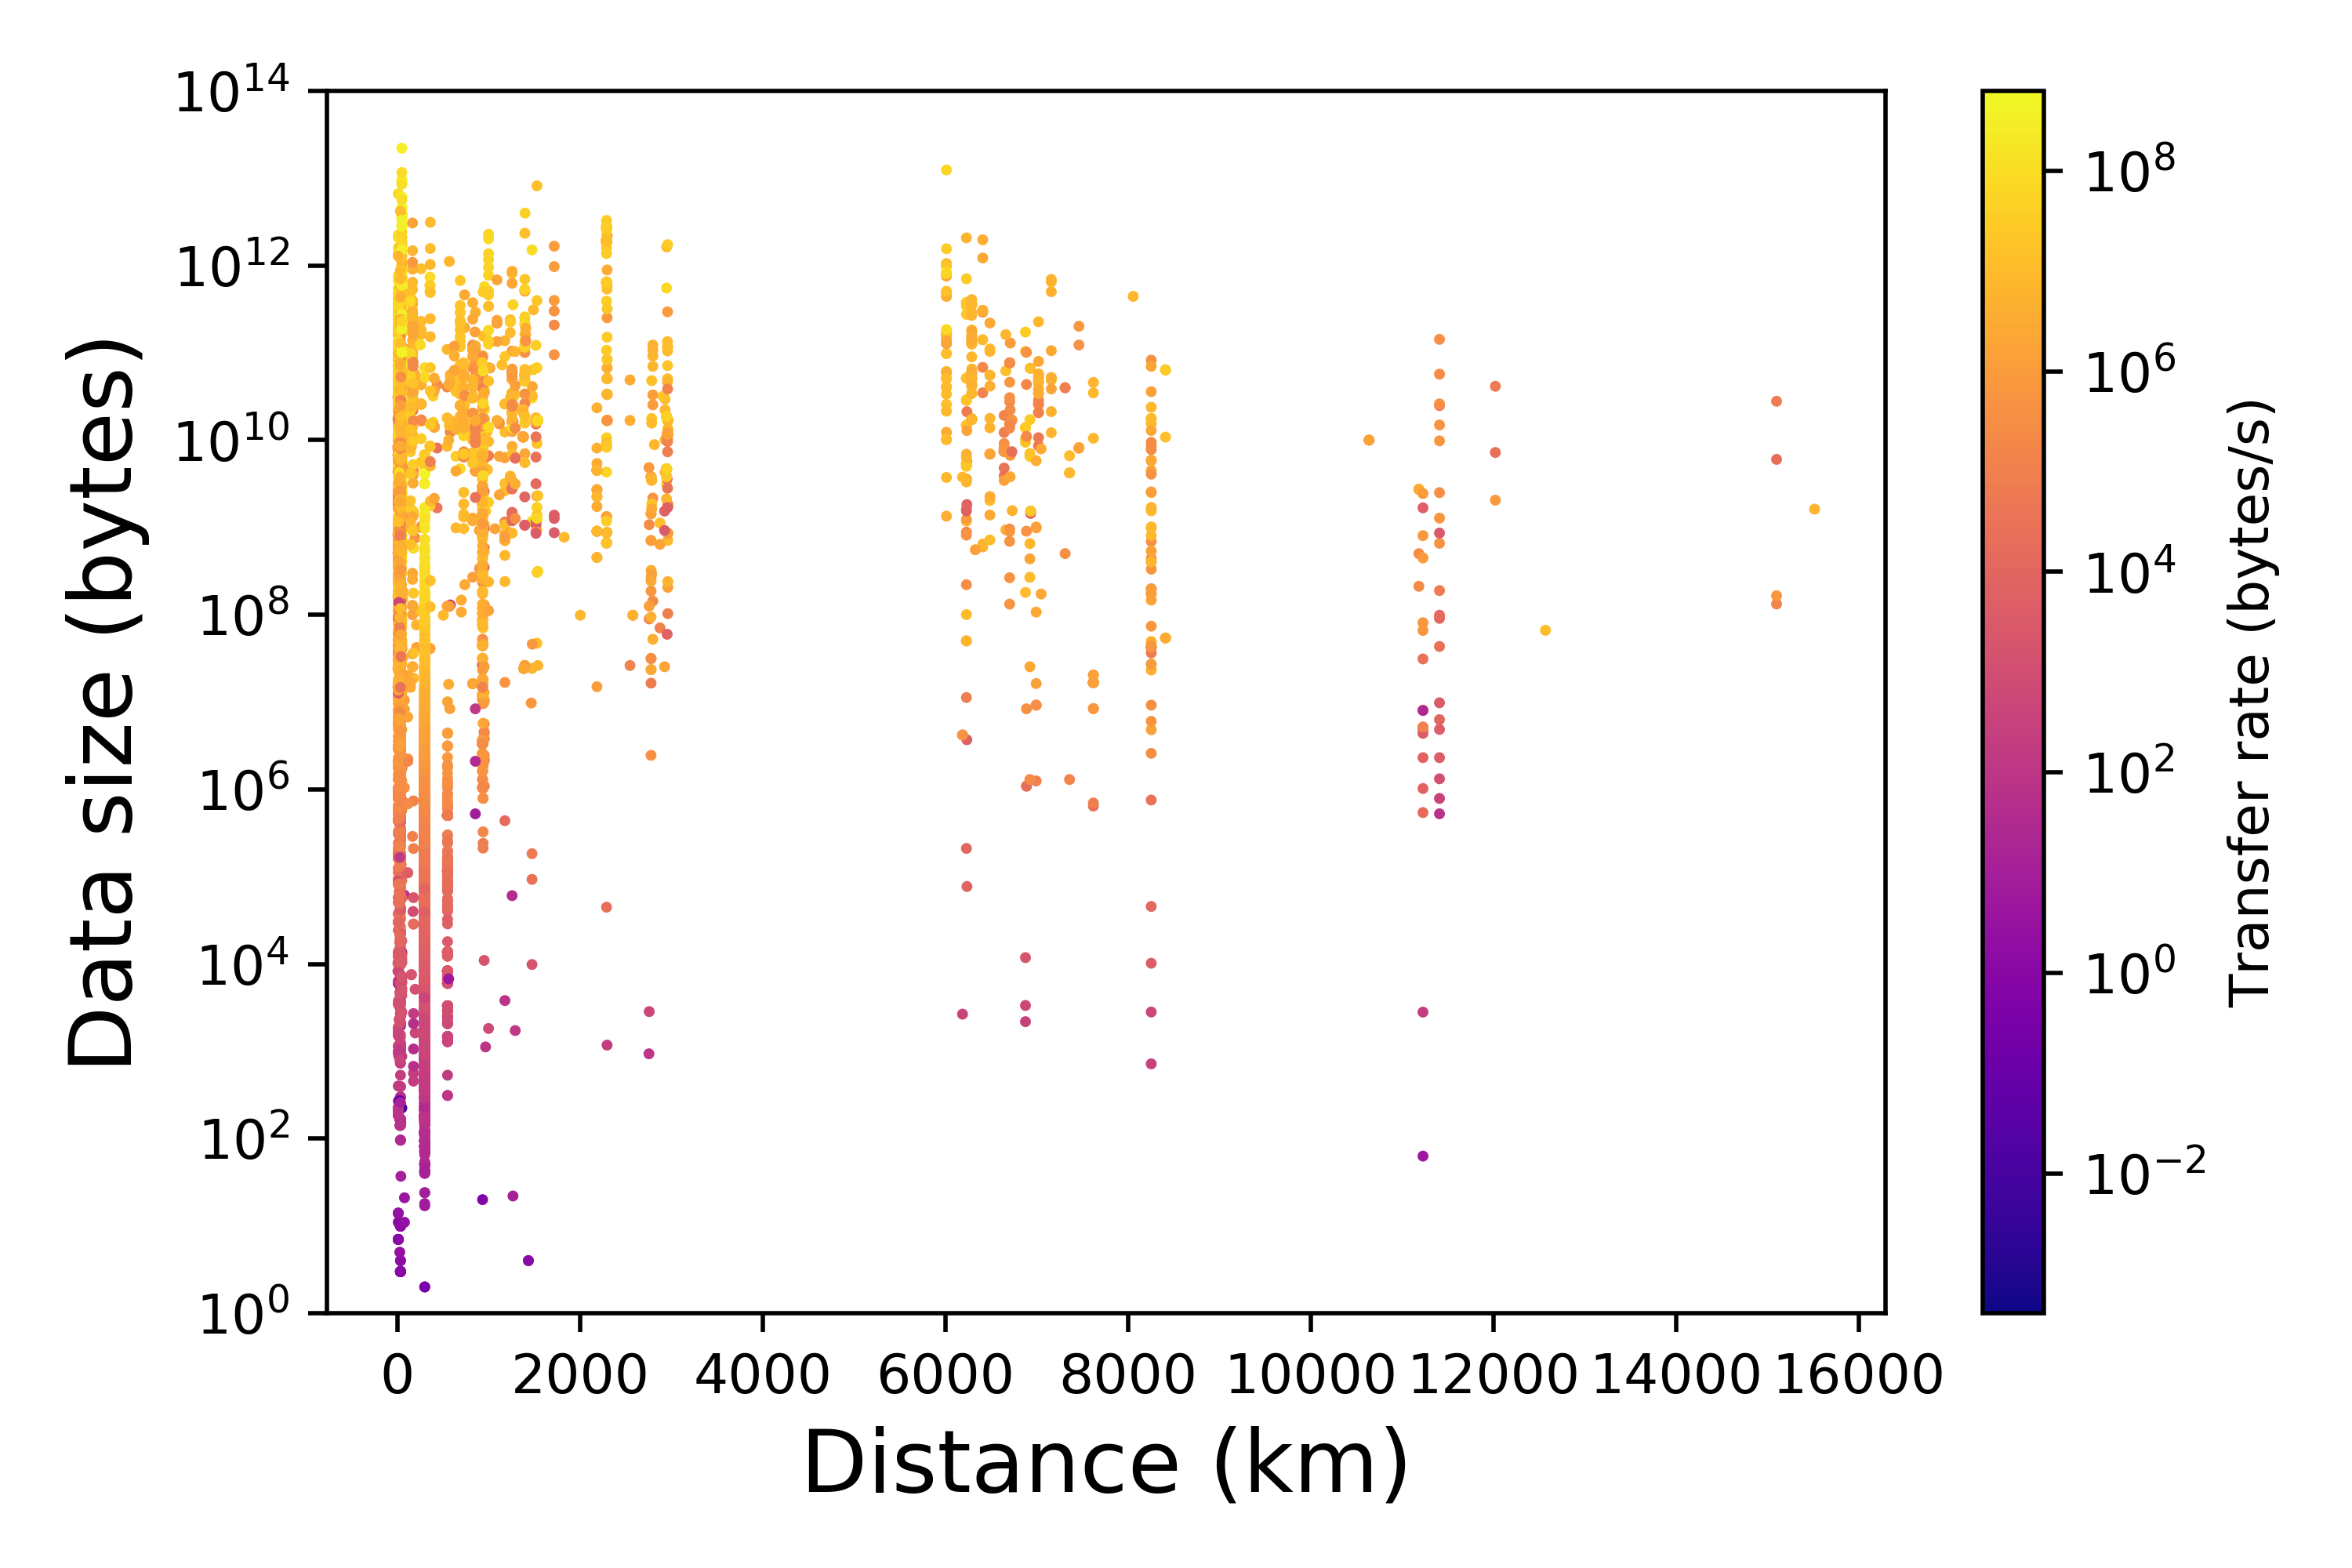
\includegraphics[trim=0.19in 0.1in 0.2in 0.1in,clip,width=\columnwidth]{Figures/size-distance-speed.png}

\vspace{-2ex}

\caption{The 80,322 transfers with Petrel as source or destination. Each
point represents a single transfer,
and gives transfer size vs.\ great circle distance between Petrel and remote source or destination, 
with transfer rate color coded.\label{fig:usage2}}
\end{figure}


\begin{figure}
\centering
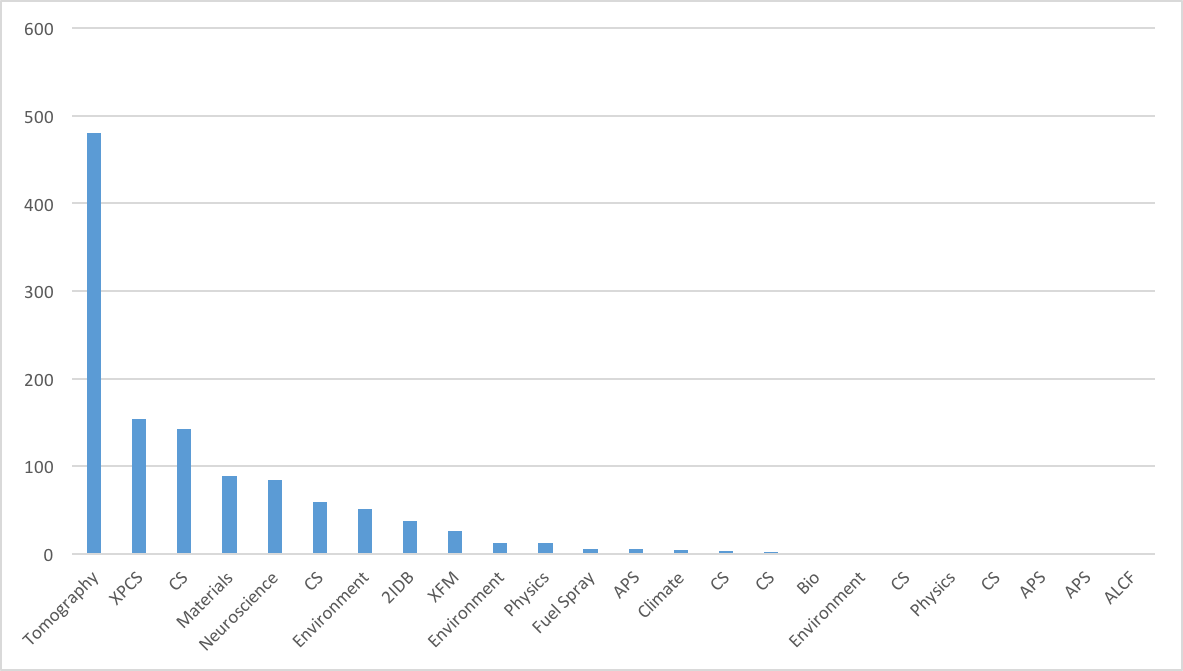
\includegraphics[trim=0.1in 0.1in 0.1in 0.1in,clip,width=\columnwidth]{Figures/usage.png}

\vspace{-2ex}

\caption{TBD\ian{to improve if we want to include it.}.\label{fig:usage3}}
\end{figure}



\section{Related Work}

Distributed file system ... e.g., AFS 

The Data Capacitor~\cite{simms2007empowering}

wide area file system: Andrew File System~\cite{howard1988scale}, Lustre on TeraGrid~\cite{simms2007wide}

Logistical networking~\cite{beck2000logistical} 




\section{Conclusions}


Today Petrel allows the easy sharing of data with colleagues and the community.
In the future our plan is to enhance Petrel to be able to support the analysis of the data by the same sharing group:
starting with defined analysis infrastructure and over time moving to more generic analysis infrastructure.

\section*{Acknowledgments}
The Argonne Leadership Computing Facility is a DOE Office of Science User Facility supported under contract DE-AC02-06CH11357.


\bibliographystyle{ACM-Reference-Format}
\bibliography{petrel} 

\end{document}
